\documentclass[10pt,a4paper]{jarticle}
\usepackage{docmute}
\usepackage{tc2016_utf}
\usepackage[dvipdfmx]{graphicx,color}
\usepackage[fleqn]{amsmath}
\usepackage{algorithm,algorithmic}
\usepackage{amssymb,epsfig}
\usepackage{ascmac}

\usepackage{url}
\usepackage{bm}
\usepackage{ascmac}
\usepackage{pifont}
%\usepackage{multirow}
\usepackage{enumerate}
%\usepackage{cases}
\usepackage{type1cm}
\usepackage{here}
\usepackage{secdot}
\sectiondot{subsection}
\sectiondot{subsubsection}

\input{jdummy.def}

\def\vec#1{\mbox{\boldmath$#1$}}
\def\vector#1{\mbox{\boldmath $#1$}}

\newcommand{\argmax}{\mathop{\rm arg~max}\limits}
\newcommand{\argmin}{\mathop{\rm arg~min}\limits}
\newcommand{\umax}{\mathop{\rm max}\limits}

\def\R{{\Bbb R}}
\def\Z{{\Bbb Z}}

\renewcommand{\topfraction}{0.8}
\renewcommand{\bottomfraction}{0.8}
\renewcommand{\dbltopfraction}{0.8}
\renewcommand{\textfraction}{0.1}
\renewcommand{\floatpagefraction}{0.8}
\renewcommand{\dblfloatpagefraction}{0.8}
\setcounter{topnumber}{3}
\setcounter{bottomnumber}{3}
\setcounter{totalnumber}{3}
\begin{document}
\section{物理シミュレータの活用}
\label{sec:simulation}

これまで述べた様々な機能の開発を効率化するべく,ROS 標準の物理シミュレータ Gazebo を活用した.シミュレータを利用することで,実機で動作させる前段階においても机上で動作検証が可能となった.さらに,九州からつくばへのロボット搬送期間においても,デバッグ作業を継続することができたことも,遠方からの参加チームとしては特筆すべき利点であった.

本Gazebo 対応に際して,1) シミュレーションモデルの構築,2) ros\_control への対応,を主として行った.本節ではこれらについて説明する.

\subsection{シミュレーションモデルの構築}
\label{subsec:simulationmodel}
Gazebo 上でロボットの動作を模擬するために主として,1) ロボットモデル,2) 走行フィールド,3) 人物モデル,というシミュレーション用のモデルを構築した.これらを統合して構築したシミュレーション空間を,Fig.\ref{142629_6Dec16}に示す.以下では,各構成要素について順に述べる.

1) ロボットモデルについては,3D CAD ツールによって作成した.本ロボットモデルを Gazebo 上に表示させた際の様子をFig.\ref{142629_6Dec16}に示す.

2) 走行フィールドについては,機能の検証をすることが目的であるため,つくばチャレンジと同一の仮想空間を構築する必要は無いと判断した.また,フィールドを一から構築するには多大な工数を要するため,既存の仮想環境を利用することで開発効率の向上を測ることとした.今回我々は,既存のROS 対応ロボットHuskey に利用されているフィールドを元にカスタマイズしたものを使用した.本フィールドをFig.\ref{142629_6Dec16}に示す.当該フィールドには多様な形状の障害物が随所に配置されているという特長を有しており,障害物の回避時や人物探索時のご検出挙動の傾向を把握する上で有効であると判断したためである.

3) 人物モデルについては,人物探索の精度や,探索対象アプローチの挙動を,シミュレーション空間上で評価するために構築した.当該人物モデルをFig. \ref{142629_6Dec16} に示す.今回は点群情報のみを用いて人物探索をしているため,寸法や形状の再現を優先した設計を行ったが,色情報や反射強度といった形状以外のパラメータの設定については特段の設計は行わないこととした.

\begin{figure}[ht]
    \centering
    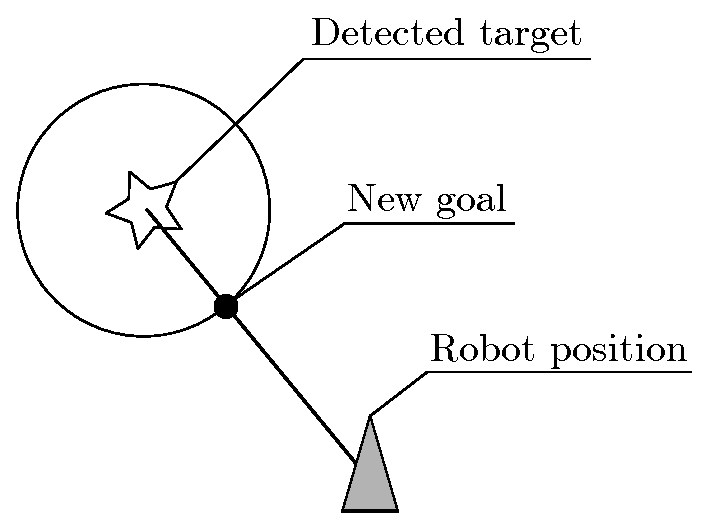
\includegraphics[width=5cm]{./fig/eps/approach_to_target.eps}
    \caption{探索対象へのアプローチ}
    \label{142629_6Dec16}
\end{figure}

\subsection{ros\_control への対応}
\label{subsec:ros_control}
ROS には,実機とシミュレータ間で共通のコントローラを利用できるようにする ros\_control という

\end{document}